\documentclass{include/thesisclass}
\usepackage{esvect}
\usepackage{amsthm}
\usepackage{listings}
\lstset{language=java}
\usepackage{hyperref}
\usepackage[ngerman]{babel}
% Main File - Based on thesisclass.cls
% Comments are mostly in English
% ------------------------------------------------------------------------------
% Further files in folder:
%  - include/cmds.tex (for macros and additional commands)
%  - include/kitlogo.pdf (for titlepage)
%  - lit.bib (bibtex bibliography database)
%  - include/titlepage.tex (for layout of titelpage)
% ------------------------------------------------------------------------------
% Useful Supplied Packages:
% amsmath, amssymb, mathtools, bbm, upgreek, nicefrac,
% siunitx, varioref, booktabs, graphicx, tikz, multicol





%% -------------------------
%% |    Thesis Settings    |
%% -------------------------
% english or ngerman (new german für neue deutsche Rechtschreibung statt german)
\SelectLanguage{ngerman}
% details on this thesis
\newcommand{\thesisauthor}{Kiril Voigtländer}
\newcommand{\thesistopic}{\Huge Simulation bewegter Teilchen in elektrischen und magnetischen Feldern}
\newcommand{\thesisentopic}{Name of the Topic in English}
\newcommand{\thesislongtopic}{Very long and very detailed description of the very interesting thesis topic (only necessary for pdfsubject tag).}
\newcommand{\thesisinstitute}{Otto-Kühne-Schule}
\newcommand{\thesisreviewerone}{Herr Schmalstieg}
\newcommand{\thesisreviewertwo}{}
\newcommand{\thesisadvisorone}{} % to use: enter names and uncomment in titlepg
\newcommand{\thesisadvisortwo}{}
\newcommand{\thesistimestart}{18.08.2021} % on titlepage
\newcommand{\thesistimeend}{27.10.2021} % on titlepage
\newcommand{\thesistimehandin}{27.10.2021} % on second page 'preamble'
\newcommand{\thesispagehead}{Facharbeit: \thesisentopic} % page heading
% eigene Befehlsdefinitionen:
\newcommand{\vektor}[3]{\left(\begin{array}{c}#1\\#2\\#3\end{array}\right)}
\newcommand{\m}[9]{\left(\begin{array}{ccc}
#1&#2&#3\\
#4&#5&#6\\
#7&#8&#9\\
\end{array}\right)}




%% ---------------------
%% |    PDF - Setup    |
%% ---------------------
% This information will appear embed into the PDF file as meta data, but will 
% not be printed anywhere
\hypersetup
{
    pdfauthor={\thesisauthor},
    pdftitle={Bachelorarbeit: \thesistopic},
    pdfsubject={\thesislongtopic},
    pdfkeywords={kit,physik,bachelor,thesis,\thesisauthor}
}





%% --------------------------------------
%% |    Settings for Word Separation    |
%% --------------------------------------
% Help for separation:
% In German package the following hints are additionally available:
% "- = Additional separation
% "| = Suppress ligation and possible separation (e.g. Schaf"|fell)
% "~ = Hyphenation without separation (e.g. bergauf und "~ab)
% "= = Hyphenation with separation before and after
% "" = Separation without a hyphenation (e.g. und/""oder)

% Describe separation hints here:
\hyphenation
{
    über-nom-me-nen an-ge-ge-be-nen
    %Pro-to-koll-in-stan-zen
    %Ma-na-ge-ment  Netz-werk-ele-men-ten
    %Netz-werk Netz-werk-re-ser-vie-rung
    %Netz-werk-adap-ter Fein-ju-stier-ung
    %Da-ten-strom-spe-zi-fi-ka-tion Pa-ket-rumpf
    %Kon-troll-in-stanz
}





%% -----------------------
%% |    Main Document    |
%% -----------------------
\usepackage{lipsum} % for Lorem Ipsum text example
\begin{document}
    % Titlepage and ToC
    \FrontMatter

    % coordinates for background border
\newcommand{\diameter}{20}
\newcommand{\xone}{-15}
\newcommand{\xtwo}{160}
\newcommand{\yone}{15}
\newcommand{\ytwo}{-253}




\begin{titlepage}
    % background border
    \begin{tikzpicture}[overlay]
    \draw[color=gray]
            (\xone mm, \yone mm)
      -- (\xtwo mm, \yone mm)
    arc (90:0:\diameter pt)
      -- (\xtwo mm + \diameter pt , \ytwo mm)
        -- (\xone mm + \diameter pt , \ytwo mm)
    arc (270:180:\diameter pt)
        -- (\xone mm, \yone mm);
    \end{tikzpicture}



    % KIT image and sign for faculty of physics
    \begin{textblock}{10}[0,0](4.5,2)
         \includegraphics[width=.25\textwidth]{include/PädaLogo.pdf}
    \end{textblock}
    \changefont{phv}{m}{n}    % helvetica
    \begin{textblock}{10}[0,0](5.5,2.2)
        \begin{flushright}
            \Large Leistungskurs PHYSIK\\\thesisinstitute
        \end{flushright}
    \end{textblock}



    % horizontal line
    \begin{textblock}{10}[0,0](4.2,3.1)
        \begin{tikzpicture}[overlay]
        \draw[color=gray]
                (\xone mm + 5 mm, -12 mm)
          -- (\xtwo mm + \diameter pt - 5 mm, -12 mm);
        \end{tikzpicture}
    \end{textblock}



    % begin of text part
    \changefont{phv}{m}{n}    % helvetica
    \centering



    % thesis topic (en and ge)
    \vspace*{3cm}
    \Huge\thesistopic\\
    \huge(\thesisentopic)\\



    % author name and institute
    \vspace*{2cm}
    \Large Facharbeit\\von\\
    \vspace*{1cm}
    \huge\thesisauthor\\
    \vspace*{1cm}
    \Large an der \thesisinstitute



    % possible frontimage - thanks to JabberWok
    % for publishing the img under GNU Document License
    \vspace*{1.5cm}
    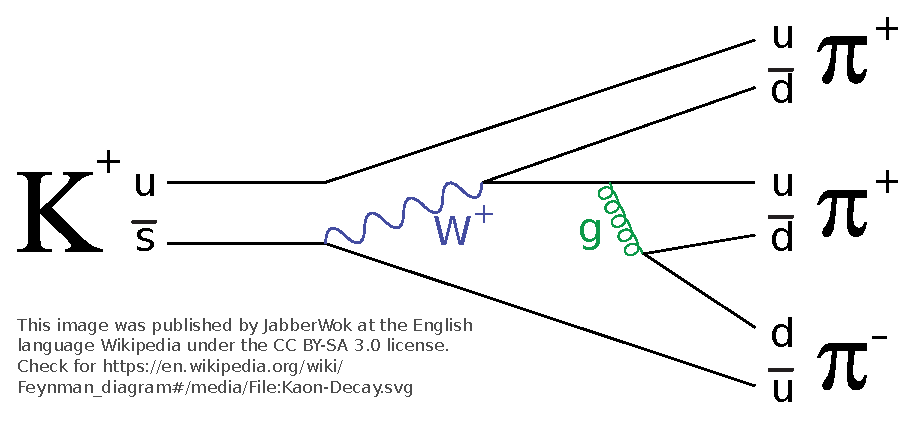
\includegraphics[scale=0.7]{./include/frontimage.eps}\\



    % examiners (Referenten)
    \vspace*{1.5cm}
    \Large
    \begin{center}
        \begin{tabular}[ht]{l c l}
        \iflanguage{english}{Reviewer}{Referent}: 
            & \hfill & \thesisreviewerone\\
        \iflanguage{english}{Second Reviewer}{Korreferent}: 
            & \hfill & \thesisreviewertwo\\
        % uncomment if you want to provide info on your advisors
        %\iflanguage{english}{Advisor}{Betreuender Mitarbeiter}: 
        %    & \hfill & \thesisadvisorone\\
        %\iflanguage{english}{Second Advisor}{Zweiter betreuender Mitarbeiter}: 
        %    & \hfill & \thesisadvisortwo\\
        \end{tabular}
    \end{center}



    % working time
    \vspace{1cm}
    \begin{center}
        \large{{Bearbeitungszeit}: \thesistimestart \hspace*{0.25cm} -- %
                                   \hspace*{0.25cm} \thesistimeend}
    \end{center}



    % lowest text blocks concerning the KIT
    \begin{textblock}{10}[0,0](4,16.8)
        \tiny{PÄDA -- Otto-Kühne-Schule}
    \end{textblock}
    \begin{textblock}{10}[0,0](14,16.75)
        \large{\textbf{www.kit.edu}}
    \end{textblock}
\end{titlepage}

    

    %\begingroup \let\clearpage\relax    % in order to avoid listoffigures and
    \tableofcontents                    % listoftables on new pages
    \listoffigures
    %\listoftables
    %\endgroup
    %\cleardoublepage


    % Contents
    \MainMatter

    \chapter{Einleitung}
    \label{chap:Einleitung}
    Die vorliegende Facharbeit befasst sich mit dem Modell des Röhrenfernsehers.
Röhrenfernseher sind Geräte, bei welchen ein Bild durch entweder einer elektrischen oder einer magnetischen Ablenkung auf einen Bildschirm gelenkt werden.
Des Weiteren wird der Röhrenfernseher in der dazu gelegten Animation bildlich dargestellt.
Sowohl die Animation als auch ihre physikalischen Eigenschaften werden in dem Kapitel \ref{chap:sim} erläutert.
Im ersten Kapitel nach der Einleitung wird die Theorie des E-Feldes und des B-Feldes betrachtet.
Für das E-Feld wichtig ist, dass es eine Ladung gibt, da um jede Ladung ein elektrisches Feld gibt.
Des Weiteren wird die Herleitung der Coulombkraft betrachtet.
Anschließend folgt eine genauere Betrachtung eines Plattenkondensators, welcher einen Spezialfall eines elektrischen Feldes darstellt.
Dabei wird auf die Formel für die Kapazität "`$C$"' und für die gespeicherte Energie im Plattenkondensator betrachtet.
Dies geschieht im Kapitel \ref{sec:Plattenkondensator}.
Für das B-Feld ist der Magnetismus wichtig, welcher zu der Entstehung des B-Feldes führt.
Hier wird die Herleitung der Lorentzkraft getätigt.
Anschließend folgt eine genauere Betrachtung des Fadenstrahlrohrs, welcher zur der Bestimmung der spezifischen Ladung "`$\frac{e}{m}$"' benutzt wird.
Diese Betrachtung geschieht im Kapitel \ref{sec:Fadenstrahlrohr}.
Des Weiteren wird die Wechselwirkung der beiden Felder aufeinander betrachtet.
%genauer erklären was passiert. geht erst nach der stunde mit dem tutor und nachdem schreiben des Kapitels
Dies geschieht im Kapitel \ref{sec:Maxwell}.
Das folgende Kapitel \ref{chap:fern} ist in zwei Unterkapitel aufgeteilt.
Im ersten Unterkapitel \ref{sec:aufbau} wird der Aufbau der Fernsehröhre betrachtet.
Dabei ist wichtig zu beachten, dass ein Röhrenfernseher aus einer Einrichtung besteht, welche die Elektronen emittiert, einer Einrichtung, welche die Elektronen steuert, eine Einrichtung, welche die Elektronen ablenkt und ein Bildschirm, wo die Elektronen als Strahl auf einen Punkt treffen, wo das Bild erzeugt wird.
Die Ablenkung kann sowohl magnetisch als auch elektrisch sein.
Die Funktionsweise der Fernsehröhre wird im Kapitel \ref{sec:Funktionsweise} behandelt.
In diesem Kapitel wird des Weiteren auch erklärt, welche Kräfte auf das jeweilige Elektron in der jeweiligen Einrichtung wirken und welche Resultate dies mit sich zieht.
Als nächstes wird die Umsetzung der Fernsehröhre in die Animation betrachtet.
Dafür wird der Code der Animation betrachtet und erläutert.
Des Weiteren ist stets eine physikalische Erläuterung dabei, welche die Prozesse beschreibt die in der jeweiligen Einrichtung geschehen.

    \chapter{Theoretischer Hintergrund}
    \label{chap:Theorie}
    In diesem Kapitel werden das E- und B-Feld betrachtet.
Des Weiteren wird ihre Wechselwirkung betrachtet.
%\section{E-Feld}
%\subsection{Entstehung und Beschreibung}
\section{Entstehung und Beschreibung des E-Feldes}
Jede Ladung wird von einem elektrischen Feld umgeben.
Zuerst muss der Begriff von Ladung geklärt werden:
Ladung ist eine Eigenschaft von Materie.
Die Einheit der Ladung ist $1C$ (Coulomb).
Alle bisherigen Experimente legen nahe, dass es nur 2 Arten von elektrischer Ladung gibt; Positiv und Negativ.
Eine Ladung bewirkt eine Kraft auf eine andere Ladung.
Gleich geladene Ladungen stoßen sich ab, während entgegengesetzt geladene Ladungen sich anziehen.
Diese Kraft wird als elektrische Kraft bezeichnet oder genauer als Coulomb-Kraft.
Die Richtung der Feldlinien ist immer die Richtung der Kraftwirkung auf einen positiv geladenen Probekörper.
Der experimentelle Nachweis der Coulomb-Kraft sieht wie folgt aus:
Man nehme sich zwei Punktladungen, welche mit $q_1$ und $q_2$ bezeichnet werden. 
Des Weiteren ist ein Abstand $r$ zwischen den Ladungen vorhanden.
Es gibt einmal die Kraft von $q_1$ auf $q_2$ ($\vv{F_{12}}$) und einmal die Kraft von $q_2$ auf $q_1$ ($\vv{F_{21}}$).
\begin{equation*}
%\label{eq:F_el}
   F_{el} = \frac{1}{4 \cdot \pi \cdot \epsilon_r} \cdot \frac{q_1 \cdot q_2}{r^2}    
\end{equation*}
Dabei stellt $\epsilon_r$ eine Materialeigenschaft dar.
Durch Betrachten der obigen Formel lässt sich schließen, dass wenn $r$ gleich bleibt, aber die Ladungen $q_1$ und $q_2$ erhöht werden, die Coulomb-Kraft ebenfalls zunimmt.
Daraus lässt sich schließen, dass die elektrische Kraft proportional zu den Ladungen $q_1$ und $q_2$ ist. 
Wenn die Ladungen $q_1$ und $q_2$ gleich bleiben und $r$ erhöht wird, dann verringert sich die elektrische Kraft.
Daraus lässt sich wiederum schließen, dass die elektrische Kraft quadratisch anti-proportional zum Abstand $r$ ist.
Diese zuvor beschriebene Kraftwirkung, lässt sich mittels Probeladungen im ganzen Raum um die Ladung messen und als Vektor an jedem Punkt visualisieren.
Diese Visualisierung des Raumes nennt man elektrisches Feld.
Die jeweilige Stärke ergibt sich aus der Größe der Probeladung $q$ und der Größe der Kraft $F_{el}$ auf die Ladung.
Die Formel für das E-Feld ist:
\begin{equation*}
%\label{eq:E}
    E = \frac{F_{el}}{q}
\end{equation*}
Die Dimension des E-Feldes lautet: $[E] = \frac{N}{C} = \frac{V}{m}$.
Veranschaulichen lässt sich die Coulombkraft durch die Animation \cite{Animation}.

%Beschreibung
Wenn ein elektrisches Feld vorhanden ist, lässt sich dieses als Eigenschaft des Raums auffassen.
Die Kraftwirkung des elektrischen Feldes wird mit Probeladung ermittelt und durch Feldlinien visuell dargestellt.
Die Feldlinien kreuzen und berühren sich nicht.
Wenn die Feldlinien eng beieinander liegen (hohe Dichte), dann ist das dort existierende elektrische Feld stark.
Wenn die Dichte der Feldlinien allerdings niedrig ist, dann ist das elektrische Feld schwach.
Es gibt zwei unterschiedliche Arten von elektrischen Feldern. 
Es gibt zum einen das homogene elektrische Feld und zum anderen das inhomogene elektrische Feld.
Bei dem homogenen elektrischen Feld stehen die Feldlinien parallel zu einander und das elektrische Feld ist an allen Stellen gleich stark.
Bei dem inhomogenen elektrischen Feld kann diese Annahme nicht getätigt werden.
% hier eventuell noch auf die verschiedene Ladungen eingehen (Punktladung, etc.)
%\subsection{Anwendung}
\section{Anwendung des E-Feldes}
\label{sec:Plattenkondensator}
Als Anwendungsbeispiel lässt sich der Plattenkondensator nehmen:
Hier lässt sich die Annahme treffen, dass das elektrische Feld zwischen den Platten homogen ist.
Allerdings muss beachtet werden, dass diese Aussage nur zwischen den Platten des Kondensators gilt, und sobald man an die Ränder des Kondensators geht, diese Aussage wegbricht.
An den Rändern wirkt nämlich ein inhomogenes elektrisches Feld.
Des Weiteren ist das elektrische Feld als $E = \frac{U}{d}$ zu bestimmen.
Somit nimmt das elektrische Feld bei einer größeren Spannung $U$ zu und bei größerem Abstand $d$ der Platten ab.
Beim Kondensator kann noch eine weitere Größe eingeführt werden, die Kapazität $C$.
Die Kapazität ist dabei so definiert, dass sie die maximale Menge an Ladung angibt, die der Kondensator auf den Platten speichern kann.
Die Herleitung ist wie folgt:
$\mbox{Flächenladungsdichte} \sigma \mbox{=} \frac{Q}{A}$.
Dies führt zum elektrischen Feld mit $\sigma = \epsilon_0 \cdot E$ als Feldgleichung.
Dabei beträgt $\epsilon_0 = 8.854 \cdot 10^{-12} \frac{As}{Vm}$ und ist unter dem Namen "`Dielektrizitätskonstante"' bekannt.
Im Allgemeinen ist das Feld auch noch vom jeweiligen Material abhängig, wodurch die Gleichung einen weiteren Term $\epsilon_r$ enthält: $\sigma = \epsilon_0 \cdot \epsilon_r \cdot E$.
Diese zusätzliche Konstante berücksichtigt dabei die spezifischen Materialeigenschaften und nennt sich "`relative Permeabilität"'.
Im Vakuum ist diese jedoch = 1.
Daraus folgt, dass $ Q = \epsilon_0 \cdot \epsilon_r \cdot \frac{A}{d} \cdot U$ ist.
Die Kapazität ist dann als
\begin{equation*}
%\label{eq:C}
    C = \frac{Q}{U} = \epsilon_0 \cdot \epsilon_r \cdot \frac{A}{d}
\end{equation*}
definiert.
%\section{B-Feld:}
%\subsection{Entstehung und Beschreibung}
\section{Entstehung und Beschreibung des B-Feldes}
Beim Nähern von 2 Magneten wurde festgestellt, dass sich gleiche Pole abstoßen und ungleiche anziehen.
Diese Kraftwirkung wurde historisch als die Magnetische Feldstärke $H$ definiert.
Das ist die eigentliche Entsprechung zum E-Feld.
Da es in der Anwendung einfacher ist, wird im Folgenden mit dem Magnetfeld das B-Feld gemeint.\footnote{In der Quelle \cite{Gente1950} wird mit der Formel $\mu_0 \cdot H$ gerechnet, während bei den verwendeten Formeln im Kapitel \ref{sec:a} mit $B$ gerechnet wird.}
Der Zusammenhang zwischen $B$ und $H$ ist wie folgt: $B = \mu_r \cdot \mu_0 \cdot H$.
Dabei ist die Dimension von $H$ : $[H] = \frac{A}{m}$.
Als Grundlage, dass ein B-Feld entsteht, muss der Magnetismus genommen werden.
Dafür muss der Begriff des Magnetismus zuerst geklärt werden.
Ein Magnet wird dadurch entmagnetisiert, dass er gestoßen oder auf einer Temperatur oberhalb der Curie-Temperatur erhitzt wird $ \approx 600 ~ ^\circ C$.
Des Weiteren führt das Durchbrechen eines Stab-Magneten in der Mitte dazu, dass zwei neue Magnete entstehen, es gibt also keine magnetischen Monopole.
Die Feldlinien eines Magneten verlaufen vom Nordpol zum Südpol.
Ein Magnetfeld bewirkt eine Kraft auf ein bewegtes geladenes Teilchen.
Die wirkende Kraft wird als magnetische Kraft bezeichnet oder als Lorentzkraft, wenn es sich um einen einzelnen Ladungsträger handelt.
Die Herleitung der Lorentzkraft sieht wie folgt aus:
Man nehme sich einen Ladungsträger (negativ) und einen langen Leiter.
Die Formel für die magnetische Kraft lautet: $F_{mag} =  B \cdot I_L \cdot \Delta l$.
Der Strom $I_L$ kann durch $\frac{\Delta Q}{\Delta t}$ ersetzt werden.
Dadurch kommt die Formel $F_{mag} = B \cdot \frac{\Delta Q}{\Delta t} \cdot \Delta l$ heraus.
Als nächstes lässt sich $\Delta Q$ durch $N \cdot e$ ersetzen.
Dabei stellt $N$ die Menge an Elektronen dar, welche betrachtet werden.
Dies führt zu der Formel $F_{mag} = B \cdot N \cdot e \cdot \frac{\Delta l}{\Delta t}$.
Dabei lässt sich der Quotient als $v$ vereinfachen, was die Geschwindigkeit der Ladungsträger angibt.
Dadurch beträgt die Formel für die magnetische Kraft nun: $F_{mag} = B \cdot N \cdot e \cdot v$.
Allerdings soll die Lorentzkraft hergeleitet werden, welche die Kraft auf einen einzelnen Ladungsträger darstellt, weshalb die magnetische Kraft mit $N$ dividiert werden muss.
Dies führt dazu, dass die Formel für die Lorentzkraft $F_L = B \cdot e \cdot v$ ist.
Diese Herleitung lässt sich prinzipiell für jede beliebige Ladung benutzen, weshalb $e$ durch $q$ ersetzt werden kann.
Daraus ergibt sich die Formel:
\begin{equation*}
%\label{eq:F_l1}
    F_L = q \cdot B \cdot v
\end{equation*}
Hier wird angenommen, dass der Geschwindigkeitsvektor senkrecht auf dem Vektor der Flussdichte steht.
Ist dies nicht der Fall, kann die Formel mit $\sin(\alpha)$ multipliziert werden, wobei alpha den Winkel zwischen den beiden Vektoren darstellt.
Der Vektor der Lorentzkraft steht senkrecht auf der durch den Geschwindigkeitsvektor und den Vektor der Flussdichte aufgespannten Ebene \cite{Lorentzkraft}.

Magnetfelder entstehen in der Gegenwart von Dauermagneten (bestehend aus Eisen, Kobalt, Nickel oder deren Legierungen) oder in der Umgebung von stromdurchflossenen Leitern. 
Die Größe der magnetischen Flussdichte $B$ ist den magnetischen Feldlinien zugeordnet.
Sie ist durch die Kraft definiert, welche ein stromdurchflossener Leiter erfährt.
Die Visualisierung des Raums, in welchem das Magnetfeld wirkt, nennt man magnetisches Feld.
Die jeweilige Stärke ergibt sich aus der Größe der Kraft $F_L$, der Länge des Leiters $l$ und der Stärke des elektrischen Stroms $I$.
Die Formel für das B-Feld ist:
\begin{equation*}
%\label{eq:B}
    B = \frac{F_L}{I \cdot l}
\end{equation*}
Die Dimension des B-Feldes lautet: $[B] = \frac{N}{Am} = \frac{Vs}{m^2} = T$.
Dabei steht $T$ für Tesla und stellt die Einheit für die Stärke des Magnetfeldes dar.

% Beschreibung von B-Feld
Wenn ein magnetisches Feld vorhanden ist, lässt sich dieses als Eigenschaft des Raums auffassen.
Die Feldlinien kreuzen und berühren sich nicht.
Des Weiteren haben Sie keinen Anfangspunkt und keinen Endpunkt, sondern sind stets geschlossen.
Wenn die Dichte an Feldlinien groß ist, dann ist die Magnetfeldstärke dementsprechend ebenfalls stark.
Wenn die Dichte an Feldlinien gering ist, dann ist die Magnetfeldstärke ebenfalls gering.
Es gibt verschiedene Magnete mit dementsprechend auch verschiedenen Formen von Magnetfeldern. 
Zum einen liegt der Stabmagnet vor, bei welchem das magnetische Feld analog zum elektrischen Feld eines Dipols ist.
Zum anderen liegt der Hufeisenmagnet vor, bei welchem im Inneren das Feld gleich wie das elektrische Feld beim Plattenkondensator aussieht.
Bei diesem ist also das magnetische Feld im Inneren homogen, allerdings an den Rändern inhomogen. 
%\subsection{Anwendung}
\section{Anwendung des B-Feldes}
\label{sec:Fadenstrahlrohr}
Als Anwendungsbeispiel lässt sich das Fadenstrahlrohr nehmen.
Hier lässt sich die Annahme treffen, dass das magnetische Feld im Inneren einer Helmholtz-Spule homogen ist. Des Weiteren gelangen die betrachteten Elektronen mit einer Geschwindigkeit von 
\begin{equation}
\label{eq:v1}
    v=\sqrt{\frac{2 \cdot e \cdot U_B}{m}}
\end{equation}
in die Helmholtz-Spule.\footnote{Diese Formel wird weiter hinten in der Arbeit hergeleitet, siehe Formel (\ref{eq:v}) dort.}
Die Elektronen wurden davor in einer Elektronenkanone freigesetzt.
Dies ist in Kapitel \ref{sec:tolle-section} dargestellt. 
Das Fadenstrahlrohr kann verwendet werden, um die spezifische Ladung $\frac{e}{m}$ eines Elektrons oder eines Ions zu bestimmen.
Dafür kann man durch die Linke-Hand-Regel die Richtung der Ablenkung eines einzelnes Elektrons im Magnetfeld bestimmen.
Dabei zeigt der Daumen die Richtung der Geschwindigkeit der negativen Ladungsträger an, der Zeigefinger die Richtung der Feldlinien und der Mittelfinger die senkrecht dazu wirkende Lorentzkraft.
Wenn nun also ein Elektron senkrecht zu den Feldlinien in ein Magnetfeld eintritt, kommt man zu dem Schluss, dass die Elektronen auf einer Kreisbahn abgelenkt werden. 
Dadurch wirkt die Lorentzkraft als Zentripetalkraft und es kann gleichgesetzt werden:
$$F_L = F_z$$
$$e \cdot v \cdot B = \frac{m \cdot v^2}{r}$$
Einsetzen von (\ref{eq:v1}) und  Umformen nach $\frac{e}{m}$ ergeben die folgende Formel.
\begin{equation*}
%\label{eq:e/m}
    \frac{e}{m} = \frac{2 \cdot U_B}{ r^2 \cdot B^2}
\end{equation*}
Diese Formel gibt die spezifische Ladung eines Elektrons an, allerdings kann man $e$ auch durch $q$ ersetzen und dadurch die spezifische Ladung eines jeden anderen Ions bestimmen, indem der jeweilige Radius beobachtet wird.
\section{Wechselwirkung der Felder}%Maxwellgleichung
\label{sec:Maxwell}
Der folgende Abschnitt bezieht sich hauptsächlich auf die Quelle \cite{Maxwell}.

Mit der Wechselwirkung zwischen den Feldern hat James Clerk Maxwell sich
beschäftigt.
Maxwell arbeitete von 1861 bis 1864 an den Gleichungen.
Er leitete die sogenannten "`Maxwell-Gleichungen"' her, welche die Zusammenhänge zwischen elektrischen und magnetischen Feldern untereinander und den Zusammenhang mit elektrischem Strom und elektrischer Ladung beschreiben.
Wenn die Lorentzkraft noch dazu genommen wird, dann kann die gesamte klassische Elektrodynamik erklärt werden.

Als erstes wird die Wechselwirkung von statischen Feldern betrachtet.
Dabei sind die elektrischen und magnetischen Felder konstant und überlagern sich ungestört.
Dabei gilt für die Kraft die Formel: $F_{Ges} = Q (E + v \times B)$.
Hier ist sowohl die elektrische als auch die Lorentzkraft wiederzufinden.
Die Lorentzkraft ergibt sich, wenn die Stärke des elektrischen Feldes $E$ gleich null ist.
Die Formel der elektrischen Kraft hingegen entsteht, wenn die Geschwindigkeit $v$ gleich null ist.
%Denn auf bewegte Teilchen wirkt die Lorentzkraft und nicht aber die elektrische Kraft.
Es gibt keine gegenseitige Beeinflussung der Felder, wenn sie stationär sind. 
Die Beeinflussung tritt erst bei sich zeitlich verändernden Feldern auf.
Dies lässt sich mit Hilfe der sogenannten "`Maxwell-Gleichungen"' betrachten.
Diese wären:
\begin{equation}
\label{eq:div E}
    \nabla \cdot E = \frac{1}{\epsilon_o} \cdot \rho
\end{equation}
\begin{equation}
\label{eq: div B}
    \nabla \cdot B = 0
\end{equation}
\begin{equation}
\label{eq:rot E}
    \nabla \times E = - \frac{\partial B}{\partial t}
\end{equation}
\begin{equation}
\label{eq:rot B}
    \nabla \times B = \mu_0 \cdot j + \mu_0 \cdot \epsilon_0 \cdot \frac{\partial E}{\partial t}
\end{equation}
Für die Wechselwirkung zwischen elektrischen und magnetischen Feldern ist nur die Betrachtung der Gleichungen (\ref{eq:rot E}) und (\ref{eq:rot B}) notwendig.
Die ersten beiden Gleichungen dienen hier als wichtige Grundlage und beschreiben das Entstehen der beiden Felder.
Die Maxwell-Gleichungen sind wie folgt zu lesen: 
Das "`$ \nabla \cdot$"' bedeutet Divergenz und beschreibt die Quelle des E-Feldes.
Wie die rechte Seite der Gleichung (\ref{eq:div E}) zeigt, ist diese Quelle die Ladungsdichte $\rho$.
Dies bedeutet, dass die Gleichung (\ref{eq:div E}) zeigt, dass die Quelle für das E-Feld die Ladung ist.
Die Gleichung (\ref{eq: div B}) zeigt, dass das B-Feld keine Quelle hat, da es ohne Quellen keine Monopole geben kann, aus welchen das B-Feld entspringt.
Ebenso begründet diese Gleichung den stets geschlossenen Verlauf der magnetischen Feldlinie, da es keinen Anfang gibt.
Dies lässt sich am Beispiel des Stabmagneten zeigen.
Dort verlassen die Feldlinien den Magneten am Nordpol und treten am Südpol wieder ein.
Auch im Inneren laufen diese Feldlinien weiter in Richtung des Nordpols und bilden so eine geschlossene Bahn ohne Anfang und ohne Ende.
Dies ist in der Abbildung \ref{fig:stabm} zu sehen.

\begin{figure}[h]
    \centering
    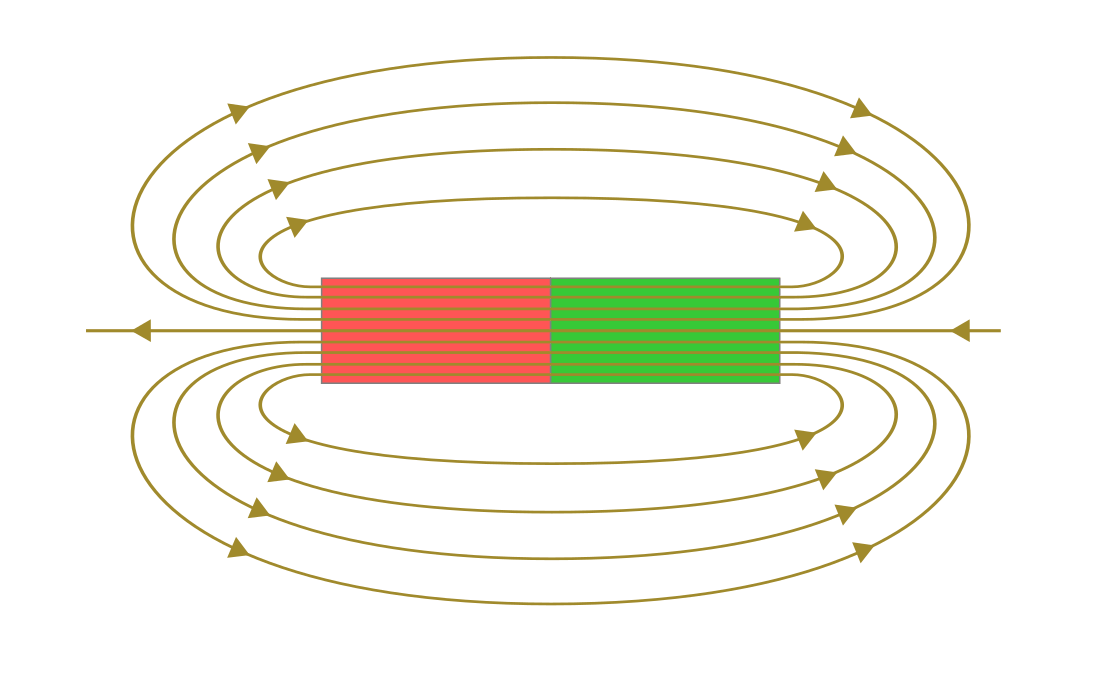
\includegraphics[width=.9\textwidth]{fig/feldlinien-stabmagnet (1).png}
    \caption{Feldlinien eines Stabmagneten (übernommen von \cite{Stabmagnet})}
    \label{fig:stabm}
\end{figure}
Die Gleichung (\ref{eq:rot E}) zeigt, dass ein entgegengesetztes sich zeitlich änderndes magnetisches Feld ein sich rotierendes elektrisches Feld erzeugt.
Das "`$ \nabla \times$"' ("`$\times$"' steht für das Kreuzprodukt) bedeutet Rotation und beschreibt die Rotation des Feldes.
Das Minus in der Gleichung und die Erklärung, dass ein entgegengesetztes magnetisches Feld entsteht, lässt sich mit Hilfe der Lentzschen Regel begründen.
Diese behauptet, dass der Induktionsstrom stets so gerichtet ist, dass er der Ursache seiner Entstehung entgegenwirkt.
Die Gleichung (\ref{eq:rot B}) zeigt, dass eine Spannung (Verschiebungsstrom) und ein sich zeitlich änderndes elektrisches Feld ein rotierendes magnetisches Feld erzeugen.
Die Formeln zeigen, dass die Wechselwirkung zwischen den Feldern ein beständiger Kreis ist. 
Ein sich veränderndes elektrisches Feld erzeugt somit ein magnetisches Feld, welches auch wiederum ein elektrisches Feld erzeugt.
Diese gegenseitige Wechselwirkung setzt sich zeitlich fort, sodass weitere Felder erzeugt werden.
Dieser Kreislauf läuft beständig weiter.


    \chapter{Fernsehröhre}
    \label{chap:fern}
     Das Kapitel bezieht sich hauptsächlich auf die Quelle \cite{Fernsehroehre}.
\section{Aufbau}
\label{sec:aufbau}
Der Kolben einer Fernsehröhre besteht aus Glas.
Dieser setzt sich aus drei Teilen zusammen: der Bildröhren-Frontplatte, dem Kolbentrichter und dem Kolbenhals.
Die Bildröhren-Frontplatte hat einen dickwandligen Preßteil, welcher mit einen hohen Rand ausgestattet ist.
Am Rand davon ergibt sich ein Preßnaht.
Der Kolbentrichter ist mit dem Anodenanschluss verbunden.
Der Kolbenhals schließt mit einem Preßteller ab, auf welchem das Strahlsystem aufgebaut ist.
Des Weiteren benötigt die Fernsehröhre eine Einrichtung, welche den Elektronenstrahl erzeugt (Elektronenkanone).
Diese Einrichtung ist wie folgt aufgebaut: Kathode, die für den Elektronenstrahl notwendige Elektronen in das Vakuum emittiert, eine Elektrode, welche die Elektronen von Kathode zum Bildschirm beschleunigt, die Einrichtung zum Steuern der Stärke des Stroms und eine Anordnung, die den Strahl bündelt, damit der Strahl als feiner Punkt auf den Bildschirm trifft. 
Die Kathode besteht aus einem einseitig geschlossenem Nickelröhrchen.
Des Weiteren ist eine Oberflächenschicht aus Barium- und Strontiumoxyd auf der geschlossenen Seite der Kathodenhülse.
In der Kathodenhülse ist eine Heizwendel, welche mit Heizstrom durchflossen ist und mit Aluminiumoxyd isoliert ist.
Die Elektronen werden mit Hilfe der positiven Spannung, welche die einzelnen Elektroden des Strahlssystem gegen die Kathode aufweisen, beschleunigt.
Als nächstes wird die Steuerelektrode für den Strahlstrom betrachtet.
Die Steuerelektrode ist auch als Wehneltzylinder bekannt.
Diese Steuerelektrode ist topfförmig aufgebaut und besitzt ein kleines kreisrundes Loch im Boden des Topfes.
Dieser Topf umgibt die Kathode, damit die emittierten Elektronen das im Topfboden befindliche Loch passieren können.
Auf die Steuerelektrode folgt die Beschleunigungselektrode.
Das Durchgangsloch der Beschleunigungselektrode ist wie von der Steuerungselektrode nicht einmal ein Millimeter groß.
Des Weiteren liegt der Abstand zwischen der Beschleunigungselektrode und der Steuerelektrode ebenfalls im Millimeterbereich.
Auf die Beschleunigungselektrode folgt eine rohrföhrmig ausgebildete Elektrode.
Hier werden die Elektronen auf ihre Endgeschwindigkeit beschleunigt.
Als nächstes Stück kommt die Linsenelektrode ran, welche dafür sorgt, dass der Strahl als feiner Punkt auf den Bildschirm trifft.
Auf die Linsenelektrode folgt eine zweite Anode, wo der Elektronenstrahl dann austritt.
Des Weiteren wird ein Bildschirm benötigt, welcher aufleuchtet, wenn dieser vom Elektronenstrahl getroffen wird.
Eine dünne Aluminiumfolie deckt die Leuchtschicht gegen das Röhreninnere ab.
Die Leuchtschicht ist über die Aluminiumfolie mit der leitenden Schicht verbunden, welche die Innenfläche das Kolbentrichters bedeckt.
Dadurch ist der Stromkreis geschlossen.
Die Aluminiumfolie muss glatt sein, damit sie nach vorne reflektieren kann.
Für die Bildröhre-Frontplatte wird eine grau eingefärbte Glasmasse verwendet, welche ungefähr 25\% des durchgehenden Lichtes absorbiert.
Und als letztes muss es entweder eine magnetische oder eine elektrische Anordnung geben.
Die elektrische Ablenkung wird durch Ablenkplatten realisiert.
Dabei gibt es zuerst eine vertikale Ablenkung und danach eine horizontale Ablenkung.
Diese Situation wird in der gegebenen Abbildung \ref{fig:Fernsehroehre} dargestellt.
Im Kapitel \ref{sec:animation} (Animation) wird mit einer magnetischen Ablenkung gearbeitet.
Dabei werden zwei Ablenkspulenpaare benutzt, wobei ebenfalls eine vertikal und eine horizontal angeordnet ist.
Wichtige Zahlenwerte für die Fernsehröhre sind zum einem die "`Diagonale"' der Bildröhren-Frontplatte und damit auf dem Bildschirm.
Der andere wichtige Zahlenwert ist der Ablenkwinkel.
Damit wird der Winkel angegeben, welcher zu der Bilddiagonalen gehört.

\section{Funktionsweise}
\label{sec:Funktionsweise}
Die Kathode, welche für das Emittieren der Elektronen zuständig ist, wird erhitzt und dabei treten Elektronen aus (glühelektrischer Effekt \ref{sec:tolle-section}).
Es wird eine Oberflächenschicht aus Barium- und Strontiumoxyd benutzt, da  dabei Elektronen bereits bei einer Temperatur von $700...800 ^\circ C$ emittiert werden.
Dies bedeutet, dass die Elektronenaustrittsarbeit für solche Materialien gering ist und deswegen gern benutzt wird.
Der Strahlstrom wird mit der Spannung zwischen der Steuerelektrode und der Kathode gesteuert.
Die Steuerelektrode wird mit einer zu der Kathode negativen Vorspannung betrieben, welche dazu führt, dass die Elektronen nicht auf der Steuerelektrode landen, sondern stets gebündelt werden.
Die Elektronen werden dazu gezwungen, zum selben Punkt zu fliegen.
Die Beschleunigungselektrode weist eine feste positive Gegenspannung zu der Kathode von einigen 1000 Volt auf. 
Die Beschleunigungselektrode hat, wie der Name bereits sagt, die Aufgabe, die Elektronen auf eine hohe Geschwindigkeit zu bringen.
Der erste Teil der Anode bewirkt mit ihrer hohen gegen die Kathode positiven Annodenspannung die Hauptbeschleunigung des Strahls.
Die Linse wirkt wegen der angelegten Spannung wie ein Engpass und führt dadurch die Elektronen zusammen, was erneut zur Bündelung des Strahls beiträgt.
Diese Fokussierung wird elektrostatische Fokussierung genannt.
Beim Auftreffen des Strahls auf den Schirm wird kinetische Energie wesentlich in Licht und Wärme umgewandelt.
Die abgebremsten Elektronen bewegen sich nun über die Aluminiumfolie als Leitungsstrom zu der positiven Hochspannungsquelle.
Da ein schwarz-weiß Bild angestrebt wird, sollen die hellen Teile des Bildes in weißem Licht aufleuchten.
Da es keinen Stoff gibt, welcher beim Elektronenaufprall weißes Licht ausstrahlt, werden verschiedene Stoffe gemischt, damit das gewünschte Weiß entsteht.
Dies führt dazu, dass auf dem Bildschirm verteilt in einem geeignetem Verhältnis gelb und blau aufleuchtende Teilchen gemischt sind.
Wenn die Ablenkung elektrisch erzeugt wird, wirkt die elektrische Kraft auf die Teilchen, welche, während sie in den Platten sind, abgelenkt werden und nachdem sie ausgetreten sind gerade auf den Bildschirm zufliegen (siehe Abbildung \ref{fig:Fernsehroehre}).
Wenn die Ablenkung allerdings magnetisch erreicht werden soll, dann wirkt die Lorentzkraft auf die Elektronen.
Dabei werden die Elektronen kreisbahnförmig abgelenkt und fliegen nach dem Verlassen des Magnetfeldes ebenfalls geradlinig auf den Bildschirm zu.
Das Bild wird beim Röhrenfernseher zeilenweise erzeugt.
Bei einem gewöhnlichen Fernseher entstehen 25 Bilder pro Sekunde.
Da bei einem Röhrenfernseher ein Bild aus 625 Zeilen besteht und damit die obere Zeile ihre Helligkeit bereits verloren hat, bis die unterste Zeile sichtbar wird, muss die Bildwechselfolge erhöht werden (z.B 50 Bilder pro Sekunde).
Das Vollbild wird in zwei Halbbilder unterteilt, welche jeweils 312,5 Zeilen haben und ineinandergeschachtelt sind.
Durch einer anliegenden Spannung, welche mit der horizontalen Ablenkspule verbunden ist, wird Strahl "`langsam"' von links nach rechts gezogen und springt dann schnell wieder nach links zurück.
Eine zweite Spannung, welche mit der vertikalen Ablenkspule verbunden ist, zieht den Strahl von oben nach unten, und wenn der Strahl unten angekommen ist, springt der Strahl wieder in die erste Zeile.
Dies lässt sich in der Abbildung auf der Seite \cite{Roehrenfernsehr} betrachten.
Dort ist der Strahlengang für die ersten 13 Zeilen dargestellt.
\begin{figure}[h]
    \centering
    \includegraphics[width=.75\textwidth]{fig/Fernsehröhre.jpg}
    \caption{Abbildung des Inneren der Fernsehröhre (übernommen von \cite{Abbildung}) }
    \label{fig:Fernsehroehre}
\end{figure}

    \chapter{Simulation}
    \label{chap:sim}
    \section{Programm}
Wie in der Abbildung \ref{fig:meineSimulation} im Anhang zu sehen ist, werden in der Simulation die Elektronenkanone, die Ablenkspulen und der Bildschirm der Fernseherröhre animiert. 
Dabei kann die Spannung der Elektronenkanone gesteuert werden und die Magnetfeldstärke ebenfalls angepasst werden.
Dadurch wird die Geschwindigkeit der Elektronen des Strahls, die Ablenkung des Strahls und schlussendlich der Auftreffpunkt jeweils dynamisch neu berechnet.
In den groß dargestellten Kreisen ist die genaue Ablenkung des Strahls durch die einzelnen Ablenkfelder dargestellt, während aufgrund der Bildauflösung am Schnittpunkt $M$ der Magnetfelder diese kreisförmige Ablenkung nicht visualisiert werden kann.   
Deswegen wird dies, wie angemerkt, in den Kreisen oben separat dargestellt.\footnote{Diese Kreise entsprechen dem grauen Kreis in Abbildung \ref{fig:ausBlog}.}
Die Geschwindigkeit, welche in den Kreisen erscheint, entspricht nicht der wirklichen Geschwindigkeit der Elektronen, da diese zu hoch ist und dadurch nicht zu sehen wäre.
Die Umsetzung des Programms erfolgt in Java mit der Greenfoot-Umgebung.
\label{sec:animation}

\section{Berechnungen zur Elektronenkanone}

%\subsection{physikalische Erklärung:}
\label{sec:tolle-section}
 
Durch die Heizspannung wird die Kathode zum Glühen gebracht, wodurch Elektronen aus der Kathode austreten (glühelektrischer Effekt).
Die Elektronen haben zu Beginn eine Geschwindigkeit von etwa $0 \frac{m}{s}$.
Im homogenen elektrischen Feld zwischen Kathode (negativ) und Anode (positiv) werden die Elektronen beschleunigt.
Dadurch fliegen die Elektronen mit zunehmender Geschwindigkeit auf die Anode zu.
Dahin werden die Elektronen durch einen Wehnelt-Zylinder auf der Mittelachse konzentriert.
Wegen dieser Richtungsfokussierung sowie ihrer erreichten Geschwindigkeit "`fliegen"' die Elektronen durch die Annodenbohrung hindurch und kommen als gebündelter und sich geradlinig bewegender Elektronenstrahl aus der Elektronenkanone hinaus.
Da die elektrische Energie in kinetische Energie umgewandelt wird, gilt laut dem Energieerhaltungssatz:
\begin{equation}
\label{eq:Energie}
   E_{kin} = E_{el}  
\end{equation}
$$ \frac{1}{2} \cdot m \cdot v^2 = e \cdot U_B$$
Diese Formel wird  nun nach $v$ umgestellt:
%\subsection{Die physikalische Formel:} 
\begin{equation}
\label{eq:v}
   v = \sqrt{\frac{2 \cdot e \cdot U_B}{m}} 
\end{equation}
%\subsection{Erklärung/Umsetzung der Physik im Code:}

Im Folgenden ist ein kurzer Auszug des Codes der Simulation dargestellt.
Zu sehen ist, dass die oben genannte Formel (\ref{eq:v}) benutzt wird und die jeweiligen Attribute aus den zugehörigen Klassen geholt werden.
Dabei wird die Spannung $U_B$ aus der Programmklasse Elektronenkanone (Objekt \lstinline$quelle$) gelesen.

\begin{lstlisting}
teilchengeschwindigkeit 
  = Math.sqrt(2 * elektronenladung * quelle.spannung * 1000 
              / elektronenmasse);
\end{lstlisting}
Die Multiplikation mit 1000 findet statt, da im Programm in Kilovolt gespeichert wird (siehe Anhang \ref{sec:Appendix}).
\section{Lorentzkraft und Ablenkung}
\label{sec:a}
%\subsection{physikalische Erklärung:}

Das Magnetfeld der Ablenkspulenpaare ist homogen und steht jeweils senkrecht zu der Bewegungsrichtung der Elektronen.
Die Elektronen kommen mit einer gewissen Geschwindigkeit $v$ aus der Elektronenkanone heraus und diese bleibt auch im weiteren Verlauf konstant.
Die Lorentzkraft $F_L$ wirkt stets senkrecht zur Bewegungsrichtung der Elektronen und der Betrag der Geschwindigkeit bleibt dadurch konstant.
Hier lässt sich die Lorentzkraft als Zentripetalkraft auffassen, da die Elektronen somit auf eine Kreisbahn abgelenkt werden (wobei der Radius dieser Kreisbahn im nächsten Abschnitt für die Berechnung der Ablenkung gebraucht wird).
Wie bereits beschrieben, wirkt die Lorentzkraft als Zentripetalkraft immer senkrecht auf die Bewegungsrichtung der Elektronen.
Dies bedeutet, dass die Kraftkomponente in Bewegungsrichtung nicht vorhanden ist und die Geschwindigkeit deswegen konstant bleibt.
Durch den Kraftansatz leitet sich ab: 
\begin{equation}
\label{eq:Kraft}
   F_L=F_z 
\end{equation}
$$ e \cdot v \cdot B = \frac{m \cdot v^2}{r}$$
Dies lässt sich nun nach $r$ umstellen und man erhält die folgende Formel.   

%\subsection{Die physikalische Formel:}

\begin{equation*}
     r = \frac{m \cdot v}{e \cdot B}
\end{equation*}

\section{Geometrische Bestimmung des Auftreffspunktes auf dem Schirm}
\label{sec:g}
Die folgenden geometrischen Erklärungen orientieren sich an \cite{Blog} und \cite{Gente1950}.
%\subsection{geometrische Erklärung:}

Die Situation ist wie in der Abbildung \ref{fig:ausBlog} dargestellt.\footnote{Eine ähnliche Abbildung befindet sich auf Seite 16 von \cite{Gente1950}.}
Um geometrisch den Ablenkwinkel zu berechnen, wird die Annahme getroffen, dass die Ablenkung des Magnetfeldes nur in einem kreisförmigen Ausschnitt wirkt.
Aus der Skizze ergibt sich, dass der Ablenkwinkel, um den der Strahl geknickt wird, gleich ist zu dem Winkel im großen Kreis zwischen den Punkten A (Eintrittspunkt in den kleinen Kreis) und B (Austrittspunkt aus dem kleinen Kreis).
Im rechtwinkligen Dreieck aus dem Punkt A und den beiden Mittelpunkten der Kreise kann man die Definition des Tangens benutzen.
Der Winkel ist $\frac{\alpha}{2}$, da die Winkelhalbierende als Verbindungslinie fungiert.
Also gilt die Formel:
\begin{equation}
    \label{eq:tan}
    \tan \left(\frac{\alpha}{2}\right) = \frac{d}{2}:r = \frac{d}{2 \cdot r}
\end{equation}
Um festzustellen, in welche Richtung um den Winkel $\alpha$ abgelenkt wird, müssen die Richtungsvektoren des Strahls und des Magnetfeldes betrachtet werden.
Die Lorentzkraft wirkt in die Richtung des Kreuzprodukts dieser beiden.
Da mit negativen Teilchen gearbeitet wird, muss der Richtungsvektor des Strahls umgedreht werden. Dadurch ergibt sich die Formel: \begin{equation}
    \label{eq:a}
    \vv{a} = - \vv{s}\times \vv{b}
\end{equation}
Um den Endpunkt auf dem Schirm zu bestimmen, kann die Skizze, aus Abbildung \ref{fig:Schirm}, zu Hilfe genommen werden.
Der Punkt $M$ stellt den Mittelpunkt des kleinen Kreises aus der Abbildung \ref{fig:ausBlog} dar.
Der Punkt $E$ stellt den Punkt dar, wo der Strahl auf den Schirm trifft.
Der Punkt $U$ hingegen stellt den Mittelpunkt des Schirms dar.
Der Winkel $\alpha$ stellt den Winkel dar, welcher sich aus der Formel (\ref{eq:tan}) ergibt und $\vv{a}$ stellt die Ablenkrichtung des Strahl dar, welche mit der Formel (\ref{eq:a}) berechnet wurde.
Da man ein rechtwinkliges Dreieck hat, kann man die Länge ausrechnen, welche die Seite $\vv{UE}$ hat.
Dies entspricht einem Vektor $\vv{v_\mathit{diff}}$, welchen man zum Ortsvektor von $U$ addieren kann.
Die Formel ist:
\begin{equation}
    \label{eq:v_d}
    \vv{v_\mathit{diff}} =  \vv{a} \cdot l \cdot \tan(\alpha)
\end{equation}
Da mit zwei Spulenpaaren gearbeitet wird, müssen die Formeln (\ref{eq:tan}), (\ref{eq:a}) und (\ref{eq:v_d}) jeweils zweimal wiederholt werden.
Nun ist der Vektor $\vv{v_\mathit{diff}}$ zweimal vorhanden, einmal für das senkrechte und einmal für das waagerechte Magnetfeld.
Diese beiden Vektoren werden auf den Punkt $U$ (Ortsvektor) hinzuaddiert, sodass sich der endgültige Punkt $E$ ergibt.
\begin{figure}
    \centering
    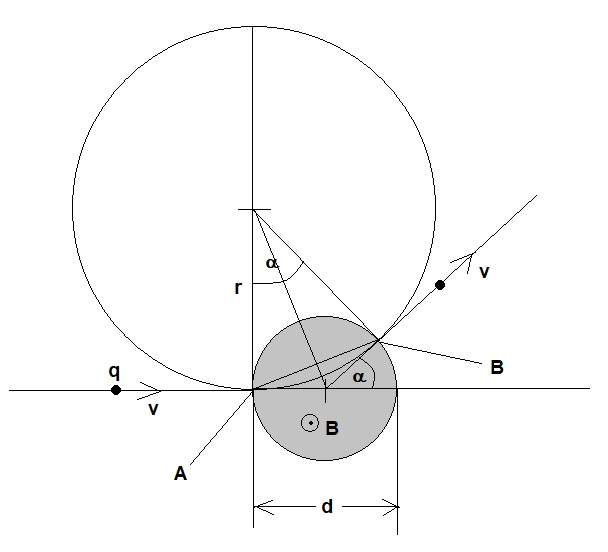
\includegraphics[width=.75\textwidth]{fig/elektronenstrahl-ablenkung_101.jpg}
    \caption{Skizze für Winkelberechnung (übernommen von \cite{Blog})}
    \label{fig:ausBlog}
\end{figure}

\begin{figure}
    \centering
    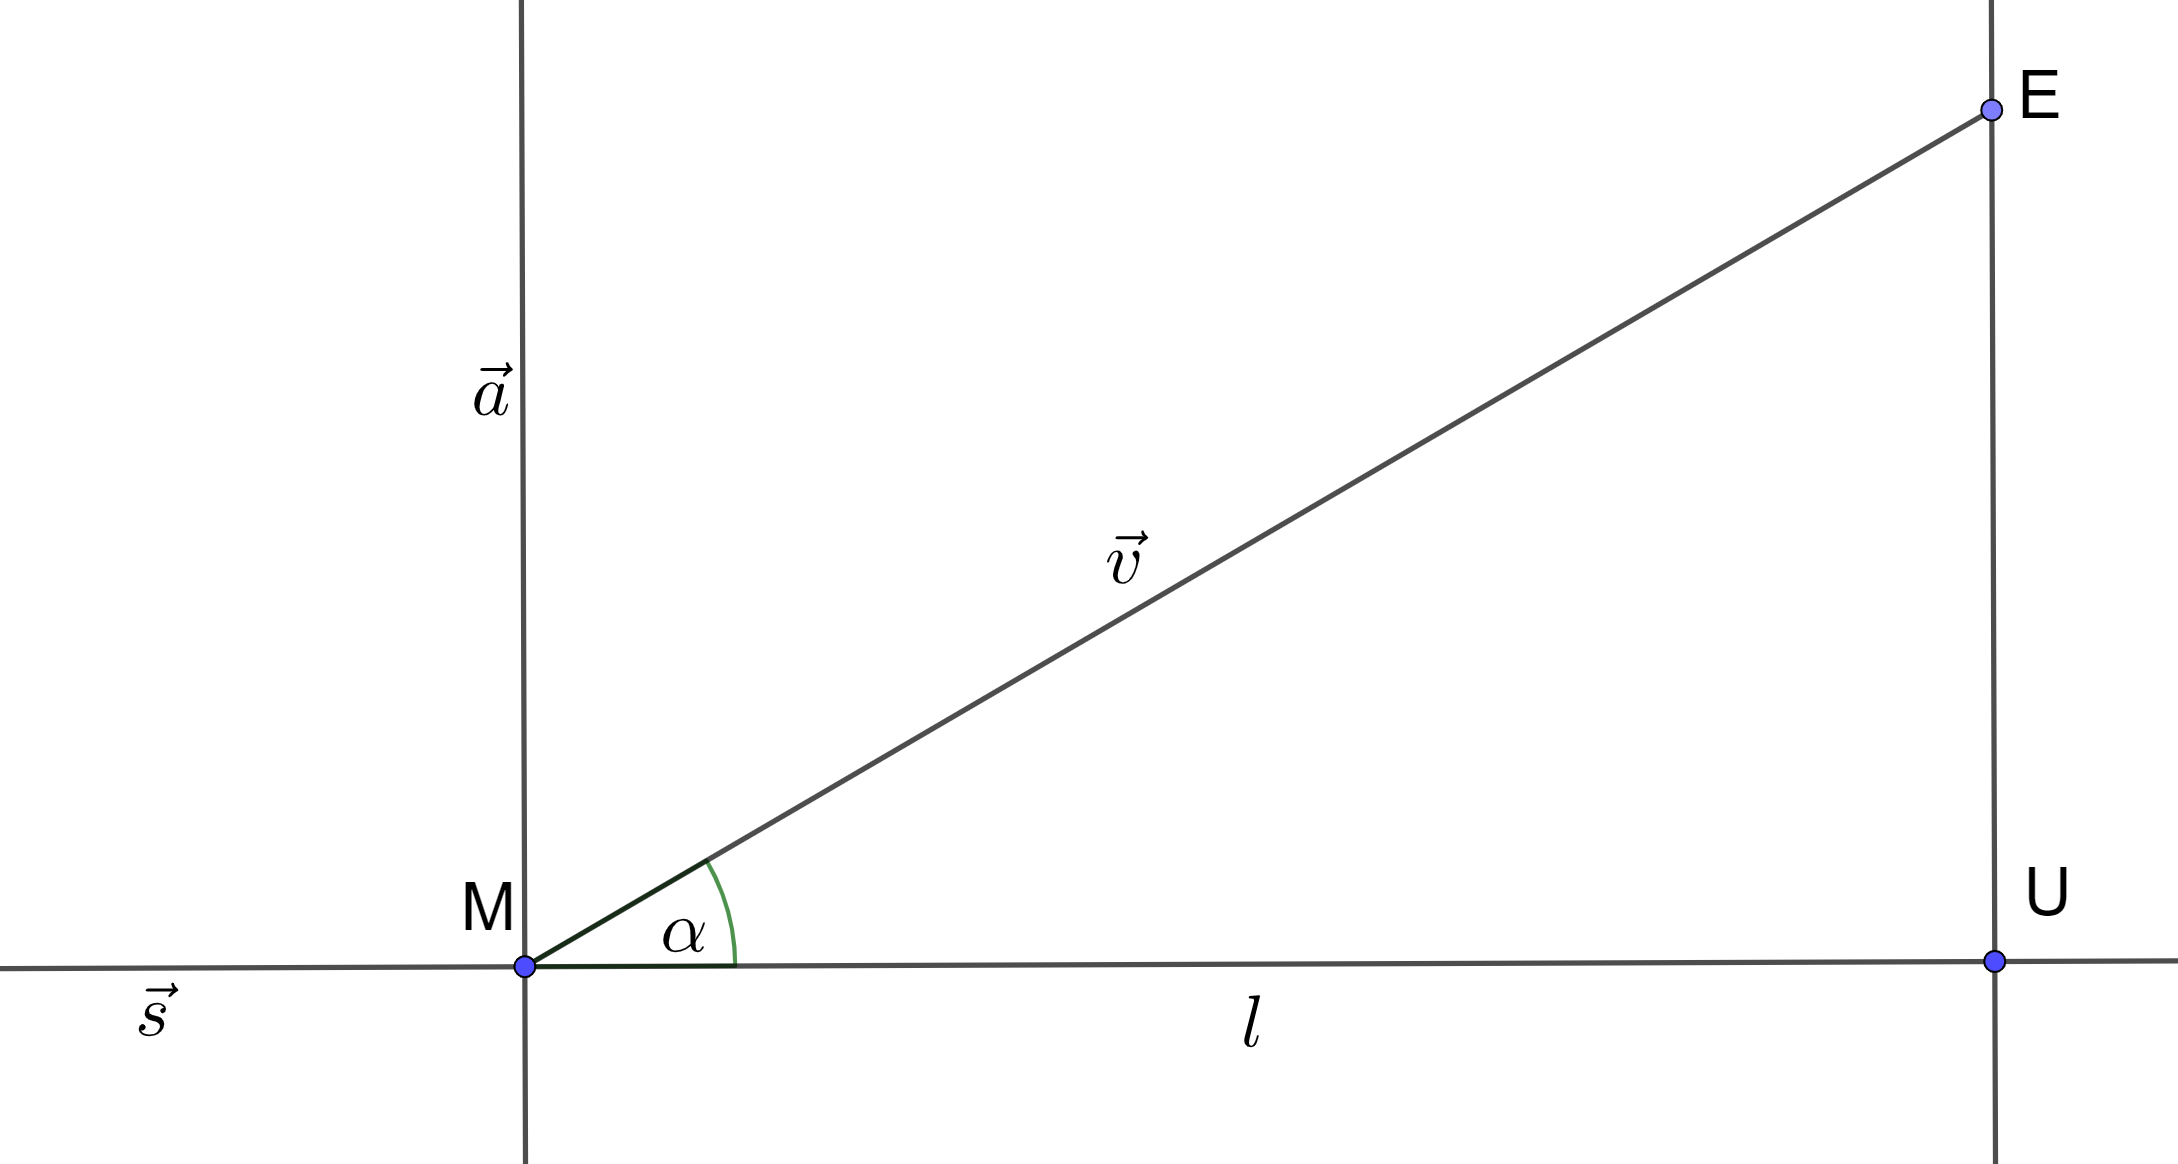
\includegraphics[width=.75\textwidth]{fig/Bildschirm_Skizze.png}
    \caption{Skizze für Auftreffen auf Bildschirm (mit GeoGebra erzeugt)}
    \label{fig:Schirm}
\end{figure}

%\subsection{Die geometrische Formel:}

%\subsection{Erklärung/Umsetzung der Physik im Code:}

Für die Umsetzung der obigen Formeln im Code wird wie folgt vorgegangen. 
Bei der Berechnung des Winkels $\alpha$ wird der arctans der oben bereits genannten Formel (\ref{eq:tan}) genommen und mit zwei multipliziert, da auf der Ausgabe der tatsächliche Winkel $\alpha$ zu sehen sein soll.
Der Winkel $\alpha$ wird im Bogenmaß berechnet, aber später in Grad ausgegeben.
Bei der \lstinline$Ablenkungsrichtung$ wird der Richtungsvektor des Strahl mit $-1$ multipliziert und danach das Kreuzprodukt mit dem Richtungsvektor des Ablenkspulenpaars gebildet, wie bereits in Formel (\ref{eq:a}) genannt.
Durch den Ausdruck \lstinline$this.richtungsvektor$ wird auf den Richtungsvektor des jeweiligen Magnetfeldes verwiesen.
Des Weiteren ist noch hinzuzufügen, dass die Berechnung jedes Ablenkspulenpaar für sich macht und daher auch eigene Werte für \lstinline$alpha$, den \lstinline$Bahnradius$ und die \lstinline$Ablenkungsrichtung$ hat.
Durch die Schleife wird bewirkt, dass wie oben bereits genannt die Berechnung des \lstinline$Ergebnisvektors$ für jedes der Spulenpaare gemacht wird.
Dies bedeutet, dass auf den \lstinline$Ergebnisvektor$, welcher zu Beginn auf den \lstinline$Bildschirmabstand$ als $x$- Koordinate, $0$ als $y$-Koordinate und 0 als $z$-Koordinate gesetzt ist, erst die Formel (\ref{eq:v_d}) benutzt wird und addiert wird.
Danach wird die Formel (\ref{eq:v_d}) erneut benutzt und erneut addiert. Dies führt dazu, dass der Punkt $E$ auf dem Schirm nun berechnet ist.

\begin{lstlisting}
alpha = 2 * Math.atan(felddurchmesser/ (2 *bahnradius ));
ablenkungsrichtung
  = strahl.quelle.richtungsvektor.
    multiplizieren(-1).
    kreuzprodukt(this.richtungsvektor);

Vektor ergebnisvektor = new Vektor(bildschirmabstand,0,0);
    for(Ablenkspulenpaar m : getWorld().getObjects(Ablenkspulenpaar.class) )
    {
        ergebnisvektor 
        = ergebnisvektor.addieren( m.ablenkungsrichtung.
        multiplizieren(bildschirmabstand*Math.tan(m.alpha)));
    }
return ergebnisvektor;

\end{lstlisting}

%\begin{tabular}{c|c|c}
    % Formel Buch & Formel Block & Anmerkungen  \\
     %\hline
    %$\alpha = \frac{d}{r}$ &$\tan(\frac{\alpha}{2}) = \frac{d}{2\cdot r}$& wegen Kleinwinkelnäherung bei dem Buch \\
    %\hline
   %$r = \frac{m\cdot v}{q\cdot B}$  & $r = \frac{m\cdot v}{q\cdot B}$& alles gleich 
     
%\end{tabular}



   % usage: \emptychapter[page displayed
                                        %        in toc]{name of the chapter}



    \chapter{Fazit}
    \label{chap:Fazit}
    Der Röhrenfernsehr dient zur einer guten Darstellung des Verhaltens von geladenen Teilchen in elektrischen und magnetischen Feldern.
Dabei lässt sich bei der Elektronenkanone der Einfluss von elektrischen Feldern beobachten.  
Durch die Ablenkspulenpaare lässt sich der Einfluss von magnetischen Feldern auf bewegte geladene Teilchen betrachten.
Beide Einrichtungen zusammen erlauben dadurch die Darstellung der wichtigen Effekte in diesem Teilgebiet der Physik.
Durch die in dieser Facharbeit erstellte Simulation lassen sich diese Effekte "`erleben"'.

In der Praxis gehört zum Fernseher mehr als nur die Bildröhre.
Zum Beispiel muss eine Ausstrahlung und Empfang eines Bildsignals durch Radiowellen oder andere Übertragungswege erfolgen.
Die dafür verwendete Physik war kein Teil dieser Arbeit.
Als Pionier für diese Aspekte des Fernsehens gilt der Physiker und Ingeneur Manfred von Ardenne (welcher nach seiner Mitarbeit am sowjetischen Atombombenprojekt jahrelang ein physikalisches Forschungsinstitut am Geburtsort des Autors dieser Facharbeit leitete).

Abschließend lässt sich anmerken, dass fast alle heutigen Fernseher nicht mehr mit der Bildröhrentechnik arbeiten.
Stattdessen kommen neue physikalische Erkenntnisse zum Einsatz, wie zum Beispiel Einsteins Photoeffekt in LED-Fernsehern.

    % appendix for more or less interesting calculations
    \Appendix
    \chapter*{\appendixname} \addcontentsline{toc}{chapter}{\appendixname}
    % to make the appendix appear in ToC without number. \appendixname = 
    % Appendix or Anhang (depending on chosen language)
    \section{Im Programm verwendete und berechnete Werte}
Neben den Naturkonstanten
\begin{itemize}
    \item Masse des Elektrons $m$ =  $9,109 \cdot 10^{-31}$ in kg
    \item Ladung des Elektrons $e$ = $1,602 \cdot 10^{-19}$ in As
\end{itemize} 
benutzt das Programm verschiedene weitere Konstanten und Einstellungsparameter. 
Diese wurden zum Teil aus \cite{Gente1950} übernommen und zum Teil durch ausprobieren mit dem Programm ermittelt, sodass die Darstellung sinnvoll wird (zum Beispiel der Strahl nicht außerhalb der Röhre landet).
Im Einzelnen sind dies:
%\section{Konstanten}
\begin{itemize}
    \item Felddurchmesser $d$ = 30 in mm
    \item Bildschirmabstand $l$ = 500 in mm
    \item Beschleunigungsspannung $U_B$ im Bereich von $12 kV$ bis $16 kV$ und  zugehöriger Richtungsvektor $\vv{s} = \vektor{1}{0}{0}$ der Beschleunigungsstrecke.
    \item Magnetfeldstärke zweier Ablenkspulen:
    \begin{itemize}
        \item $B_1$ im Bereich $-5 mT$ bis $5 mT$, zugehöriger Richtungsvektor $\vv{b_1} = \vektor{0}{0}{1}$ % senkrechte Spule
        \item $B_2$ im Bereich $-5 mT$ bis $5 mT$, zugehöriger Richtungsvektor $\vv{b_2} = \vektor{0}{-1}{0}$ % waagerechte Spule
    \end{itemize}
\end{itemize}

In Abbildung \ref{fig:meineSimulation} ist zu sehen, wie die Einstellungsparameter geändert werden können. 
Des Weiteren werden die Werte für die zu berechnenden Werte ausgegeben:
%\section{Zu berechnende Parameter}
\begin{itemize}
    \item die Energie aus dem Ansatz (\ref{eq:Energie})
    \item Teilchengeschwindigkeit $v$ in $\frac{km}{s}$
    \item die Kräfte $F_1$ und $F_2$ aus dem Ansatz (\ref{eq:Kraft}) für senkrechtes und waagerechtes Spulenpaar
    %\item Ergebnisvektor $\vv{v}$
    \item Bahnradien $r_1$ und $r_2$ in mm 
    \item Ablenkwinkel $\alpha_1$ und $\alpha_2$ in Grad (Winkel werden auch in den Kreisen sichtbar)
    %\item Ablenkungsrichtung $\vv{a}$
\end{itemize}
Der am Ende von Abschnitt \ref{sec:g} berechnete Punkt $E$ ist im Bild als Endpunkt des blauen Strahls zu erkennen.
%\section{Programm und dessen steuerung}

\begin{figure}[h]
    \centering
    \includegraphics[width=1.2\textwidth]{fig/Fernseherröhre.PNG}
    \caption{Darstellung der Simulation}
    \label{fig:meineSimulation}
\end{figure}
%\paragraph{Einstellungsparameter:}

\pagebreak
\section{\textbf{Graphische Ausarbeitung}}
Wann immer man ein Objekt (Fernseheröhre oder jedes andere mögliche Objekt) auf einen Bildschirm abbilden möchte, muss man aus 3D in der "`Realität"' 2D auf dem Bildschirm machen. Dafür muss man eine Koordinatentransformation machen, welche auch als Kameratransformation bekannt ist \cite{Kameratransformation}.

\underline{$\vv{a}$ = Blickrichtung}
$$x = \sqrt{\frac{1}{6}}$$
$$y = \sqrt{\frac{2}{3}}$$
$$z = -\sqrt{\frac{1}{6}}$$
$$\vv{a}=\vektor{\sqrt{\frac{1}{6}}}{\sqrt{\frac{2}{3}}}{-\sqrt{\frac{1}{6}}} $$
$x$, $y$ sollen positiv sein, $z$ soll negativ sein und der Betrag/Länge soll 1 sein. $X$ etwas kleiner als $y$.
$$y= \sqrt{\frac{2}{3}}$$
$$x= \sqrt{\frac{1}{6}}$$
\underline{$\vv{b}$:}
$z$ = 0 ; andere Werte so wählen, dass Skalarprodukt 0 ergibt
$$x= \sqrt{\frac{2}{3}}$$
$$y=-\sqrt{\frac{1}{6}}$$
$$z=0$$
$$|\vv{b}| = \sqrt{\frac{5}{6}}\neq 1\mbox{ ; also müssen $x$ und $y$ mit dem Kehrwert von $\sqrt{\frac{5}{6}}$, also mit $\sqrt{\frac{6}{5}}$ multipliziert werden.}$$
$$x' = \sqrt{\frac{12}{15}} = \sqrt{\frac{4}{5}}$$
$$y' = - \sqrt{\frac{1}{5}}$$
$$z' = 0$$
$$\vv{b}= \vektor{\sqrt{\frac{4}{5}}}{-\sqrt{\frac{1}{5}}}{0}$$
\underline{$\vv{c}$:}
$$\vv{c} = \vv{b}\times  \vv{a}$$
$$= \vektor{\frac{4}{5}}{-\sqrt{\frac{1}{5}}}{0}
      \times \vektor{\sqrt{\frac{1}{6}}}{\sqrt{\frac{2}{3}}}{-\sqrt{\frac{1}{6}}} \mbox{ = } 
     \left(\begin{array}{c} 
     \frac{\sqrt{5}}{5}\cdot\frac{\sqrt{6}}{6}\\2\cdot\frac{\sqrt{5}}{5}\cdot\frac{\sqrt{6}}{6}\\2\cdot\frac{\sqrt{5}}{5}\cdot\frac{\sqrt{6}}{3}+\frac{\sqrt{5}}{5}\cdot\frac{\sqrt{6}}{6}\end{array}\right)
$$
Wir suchen eine Matrix $A$, sodass

     $$A\cdot \vv{a}=\vektor{0}{1}{0}\mbox{ ist ;} $$
     $$A\cdot \vv{b}=\vektor{1}{0}{0}\mbox{ ist ;}$$
     $$A\cdot \vv{c}=\vektor{0}{0}{1}\mbox{ ist ;} $$
     
$$\mbox{$B$ = } \m{\sqrt{\frac{4}{5}}}{\sqrt{\frac{1}{6}}}{\frac{\sqrt{5}}{5} \cdot \frac{\sqrt{6}}{6}}{-\sqrt{\frac{1}{5}}}{\sqrt{\frac{2}{3}}}{2 \cdot \frac{\sqrt{5}}{5} \cdot \frac{\sqrt{6}}{6}}{0}{-\sqrt{\frac{1}{6}}}{2 \cdot \frac{\sqrt{5}}{5} \cdot \frac{\sqrt{6}}{3} + \frac{\sqrt{5}}{5} \cdot \frac{\sqrt{6}}{6}}$$
Um auf die Matrix $A$ zu kommen, muss man nun die Matrix $B$ mit Hilfe von GeoGebra invertieren:
$$\mbox{$A$ = } \m {2\cdot\frac{\sqrt{5}}{5}}{-\frac{\sqrt{5}}{5}}{0}{\frac{\sqrt{6}}{6}}{\frac{\sqrt{6}}{3}}{-\frac{\sqrt{6}}{6}}{\frac{\sqrt{30}}{30}}{\frac{\sqrt{30}}{15}}{\frac{\sqrt{30}}{6}}$$
Wir verwenden $A$, um aus einem $(x,y,z)$ Vektor $\vv{v}$ ein zweidimensionales Koordinatenpaar zu kriegen, indem wir $ A \cdot \vv{v} = \m {2\cdot\frac{\sqrt{5}}{5}}{-\frac{\sqrt{5}}{5}}{0}{\frac{\sqrt{6}}{6}}{\frac{\sqrt{6}}{3}}{-\frac{\sqrt{6}}{6}}{\frac{\sqrt{30}}{30}}{\frac{\sqrt{30}}{15}}{\frac{\sqrt{30}}{6}} \cdot \vektor{v.x}{v.y}{v.z}$ rechnen um den Vektor $ \vektor{x_1}{-}{y_1}$ rauszubekommen, wobei die $y$-Koordinate ignorieren.  
%\section{Simulation}
%\subsection{a}
%\subsection{b}
\section{zusätzliche Abbildungen}

\begin{figure}[h]
    \centering
    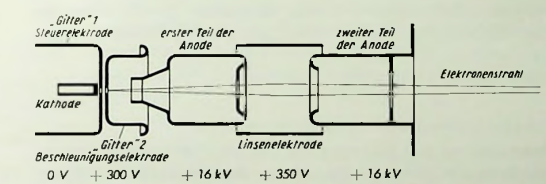
\includegraphics[width=.9\textwidth]{fig/Elektronenstrahl.PNG}
    \caption{Darstellung der Elektronenkanone (übernommen aus dem Buch \cite{Fernsehroehre})}
    \label{fig:elS}
\end{figure}

\begin{figure}[h]
    \centering
    \includegraphics[width=.75\textwidth]{fig/Fernsehröhre.jpg}
    \caption{Abbildung des Inneren der Fernsehröhre (übernommen von \cite{Abbildung}) }
    \label{fig:Fernsehroehre}
\end{figure}
 %\cleardoublepage



    % Bibliography
    \TheBibliography

    % BIBTEX
    % use if you want citations to appear even if they are not referenced to: 
    % \nocite{*} or maybe \nocite{Kon64,And59} for specific entries
    %\nocite{*}
    \bibliographystyle{babalpha}
    \bibliography{lit.bib}

    % THEBIBLIOGRAPHY
    %\begin{thebibliography}{000}
    %    \bibitem{ident}Entry into Bibliography.
    %\end{thebibliography}
    
    \chapter*{Erklärung zur Selbstständigkeit}
Ich versichere, dass ich diese Arbeit selbstständig verfasst habe und keine %
anderen als die angegebenen Quellen und Hilfsmittel benutzt habe, die %
wörtlich oder inhaltlich übernommenen Stellen als solche kenntlich gemacht habe. %und %
%die Satzung des KIT zur Sicherung guter wissenschaftlicher Praxis in der %
%gültigen Fassung vom 17.05.2010 beachtet habe.\\

\vspace{1cm}

\renewcommand{\arraystretch}{0} % for spacing in the tabular environment

\begin{flushright}
	\begin{tabular}{rr}
		Bonn, den \thesistimehandin, & \hspace*{5cm}\\[0mm]
		\cline{2-2}\\[2mm]    % the last line has height 2mm due
		& \thesisauthor       % to \arraystretch=0
	\end{tabular}
\end{flushright}

\vfill

\begin{flushright}
	Als Ansichtsexemplar genehmigt von\\
	\vspace{1cm}
	\begin{tabular}{rr}
		Bonn, den \thesistimehandin, & \hspace*{5cm}\\[0mm]
		\cline{2-2}\\[2mm]    % the last line has height 2mm due
		& \thesisreviewerone  % to \arraystretch=0
	\end{tabular}
\end{flushright}

\renewcommand{\arraystretch}{1}

%\cleardoublepage

\end{document}
